\section{Background}

\subsection{Structure of a tyre}

Tyres are composed of several layers with different functions. Figure \ref{fig:tyre_structure_diagram} by Gent et
al. \cite{Gent2005} shows the layered structure. From outer tread to inner lining, the layers are: 

\begin{description}
  \item[Tread] provides traction for driving, braking and cornering. Pattern and materials on
tread is a compromise between wear resistance, traction, handling and rolling
resistance
  \item[Belts] provide mechanical strength, impact resistance and keep tyre from expanding
under centrifugal forces.
  \item[Body ply] provides strength to contain the air pressure.
  \item[Innerliner] is a compound specifically designed to improve air retention in tyre.
\end{description}
In addition there are layers designed to improve tyre reliability, such as the belt
wedge which reduces shear between belts.


\begin{figure}[h]
\begin{center}
\includegraphics[height=8cm]{images/cited/gent2005}
\end{center}
\caption{Structure of a tyre \cite{Gent2005}.}
\label{fig:tyre_structure_diagram}
\end{figure}


In endurance testing of tyres the car is driven at test track in three shifts, until
desired number of course driving kilometers have been reached. In outdoor testing
each company has their own proprietary test protocol. Indoor testing has standards,
which mandates pressure, ambient temperature and speed as well as time driven.
According to Gent et al. \cite{Gent2005} this indoor testing takes 34 hours of driving at 120
km/h.
3
In addition to endurance testing, there is high-speed testing where tyre speed is
gradually accelerated in steps of 10 km/h at regular intervals until target speed is
reached.


\subsection{Environment inside tyre}
The energy harvester will be placed inside the tyre. Previous studies by Niskanen et al \cite{Niskanen2014}. have shown that the tyre will experience acceleration in all three axes. Tangential and centripetal accelerations are dominant, they can reach amplitudes up to 150 g in test fixture. In addition a study done by Löhndorf et al. \cite{Lohndorf2007} shows shock survival of up to 4 000 - 5 000 g is required for reliability. 

Temperature inside of the tyre will reach equilliberium in ambient + 5-10 \degree C, so operation temperature should be in range of -40 to + 75 \degree C to have some safety margin on top of usual ambient conditions. 

Previous work by Niskanen et al. \cite{Niskanen2014} was used to as a basis for analysis of characteristics of acceleration inside the tyre. Raw data was used to gather minimum and maximum values of acceleration as well as frequency components inside tyre. Data was gathered at 20 km/h, 60 km/h and 80 km/h speeds. Figure \ref{80_TD} shows time domain representations of the acceleration along 3 axes as shown in figure \ref{tyre_axes}.

\begin{figure}[htb]
\begin{center}
\includegraphics[height=4cm]{images/cited/matilainen2012}
\end{center}
\caption{Axes in measurement by Matilainen et al. \cite{Matilainen2012}}
\label{tyre_axes}
\end{figure}

Frequency domain representations were calculated in Matlab. There are two main contributors to base frequencies: first is the rotational frequency of tyre itself and second is the impact when the tyre deforms as it contacts the drum.. There is clearly visible series of frequency components spaced at the rotational frequency of tyre as well as shock harmonics at upper frequencies. Figures \ref{80_FFT} and \ref{80_FFT_zoom} show the total frequency spectrum and the dominant frequency components.

\begin{figure}[htb]
\begin{center}
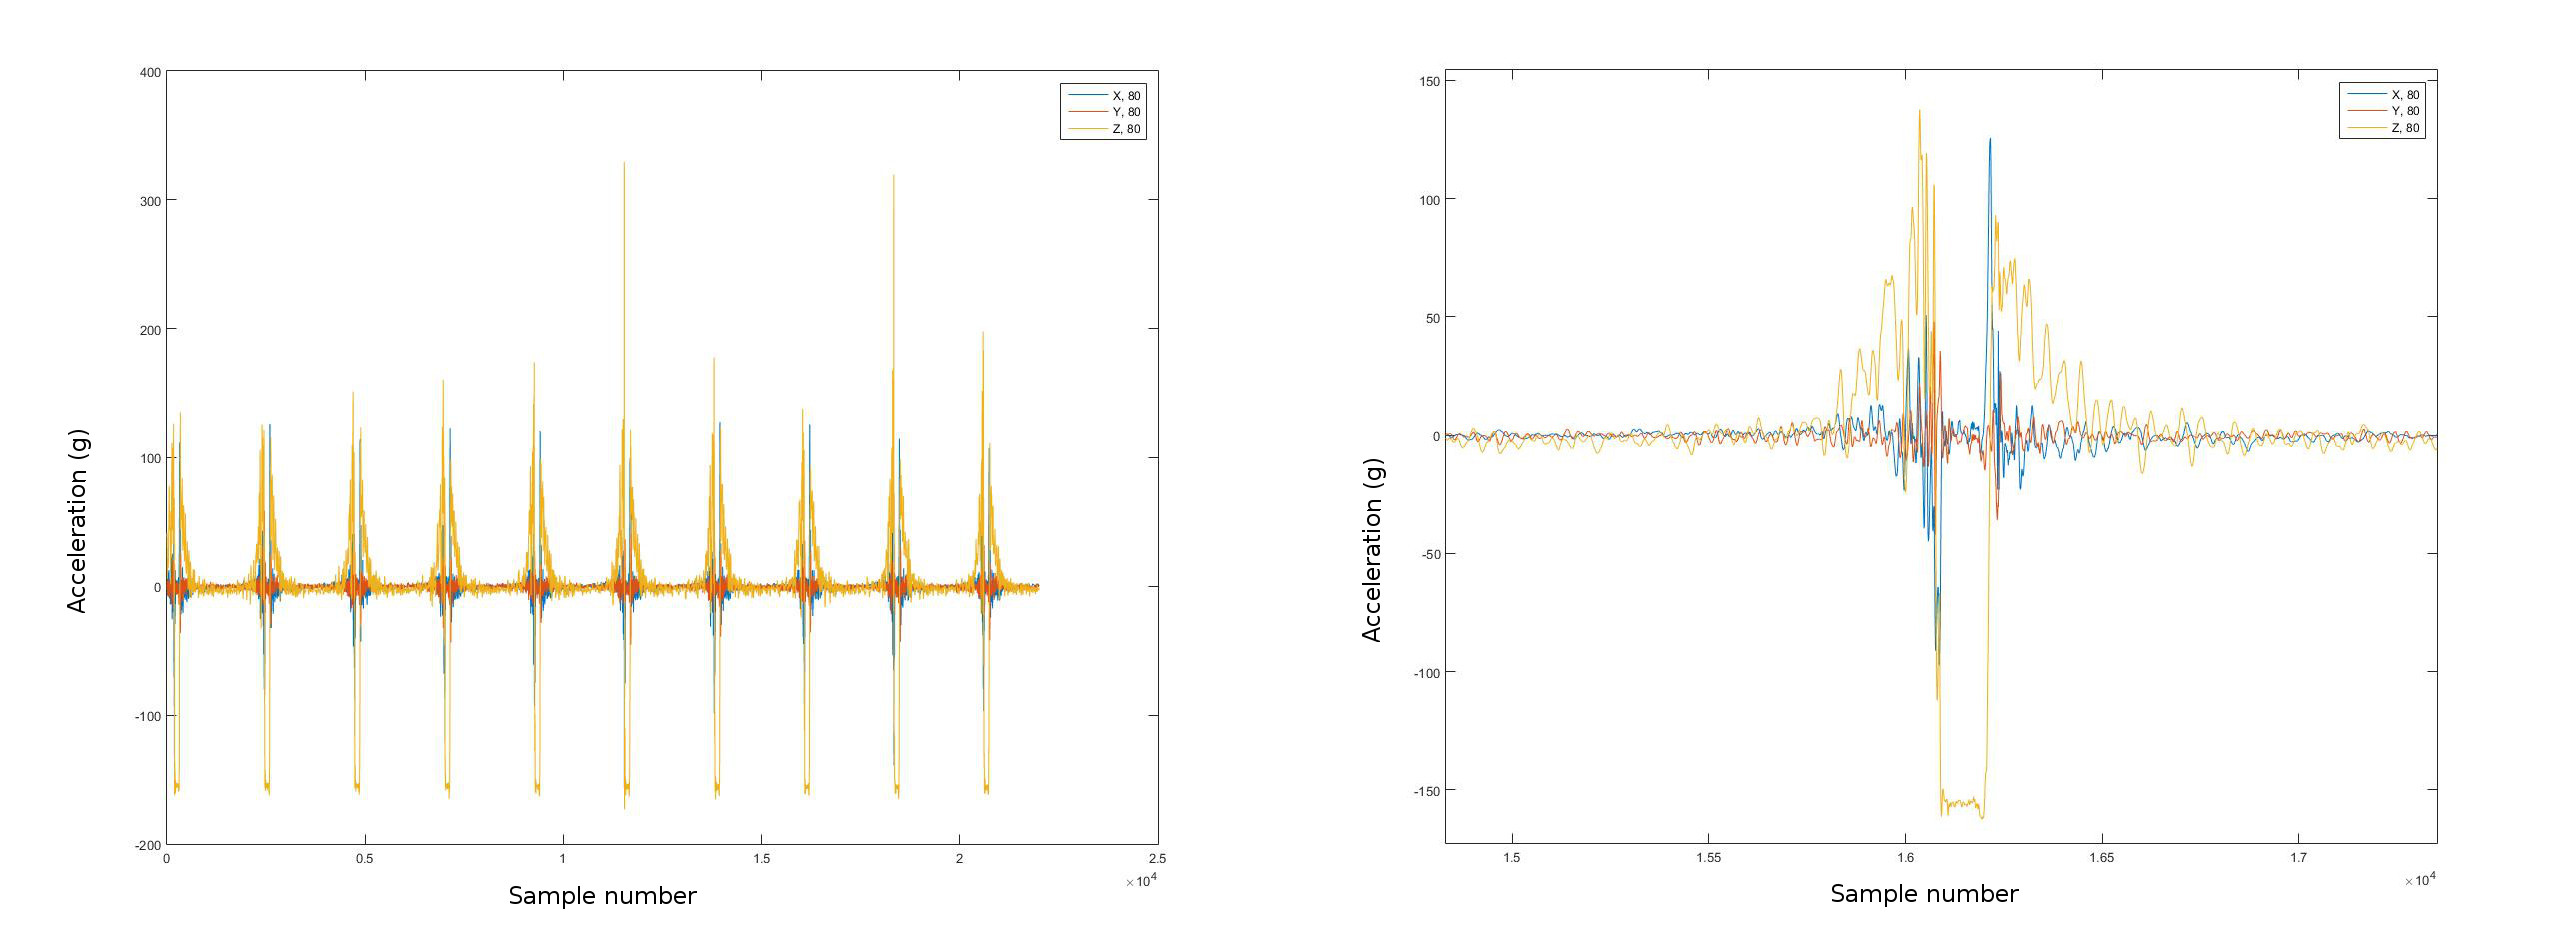
\includegraphics[height=6cm]{images/matlab_figures/80kmh_timedomain_combined}
\end{center}
\caption{Acceleration of inner lining of tyre at 80 km/h in time domain.}
\label{80_TD}
\end{figure}

\begin{figure}[htb]
\begin{center}
\includegraphics[height=4cm]{images/matlab_figures/FFT-80_combined}
\end{center}
\caption{Most of the energy is found in 10-100 Hz range.}
\label{80_FFT_zoom}
\end{figure}

It's important to notice that the sensor used was piezoelectric, which forms a highpass filter as the operation of sensor is based on charge between layers. This charge dissipates over time, so the steady-state centripetal acceleration reads as zero. Any device on the rotating tyre will experience centripetal acceleration (acceleration towrds centre of rotation) at the amplitude of: 

\begin{equation}
  a_{centripetal} = \omega^2 r,
\end{equation}

where $\omega$ is the rotation speed of tyre and $r$ is the radius of rotation.

\subsection{Energy harvesting}
\subsubsection{Overview of methods}
First step of designing a system for energy harvesting was to identify the currently known methods and their properties. Kubba et al. \cite{Kubba2014} have done a study on tyre pressure sensor technology, they present electromagnetic, electrostatic, piezoelectric and thermal solutions as possible candidates for energy harvesting. In addition, triboelectric and magnetostrictive methods have been proposed by Bowen et al \cite{Bowen2014}. Outside of the context of tyres, Paradiso et al. \cite{Paradiso2005} present solar and radiowave harvesting techniques. Radioactive power source has been suggested by Lal et al \cite{Lal2004}. 

Electromagnetic power sources are based on Faraday's law of electromagnetic induction. A magnet and a coil are put in motion relative to each other, and the changing magnetic flux through the coils of the generator produces voltage. Current through such device is determined by load resistance. Technology is widely used in power generation, where a primary power source such as wind or flow of water provides rotation for the generator. While conventional designs use rotational movement, linear generator designs exist. Boldea and Nasar \cite{Boldea1999} provide an overview of linear generator and actuator theory. 

Electrostatic devices charge plates of a capacitor and use mechanical vibration to vary the structure of the capacitor. As the capacitance value changes with the structure, energy can be harvested from increased potential energy in capacitor. Drawback of this method is the required control electronics and high polarization voltages needed for maximal efficiency. There are also electrostatic methods which use electrets. These electrects hold constant charge and polarization for years and they can be used in electrostatic harvesters which do not require an external exitation source \cite{Boisseau2012}. As electret elements and electrostatic generators are not readily available, they have been excluded from this study.

Piezoelectric materials generate charge in response of mechanical stress. This stress can be caused by firmly attaching the piezoelectric element to a surface which deforms (simply supported) or by leaving one end of the element free-hanging while other end is fixed (cantilevered). Dynamics of the generator are very different for the different configurations, Kim et al. \cite{Kim2014a} provides a model for impact-based piezoelectric harvester while Erturk et al. have done in-depth analysis of cantilevered piezoelectric modeling \cite{Erturk2009}. 

Thermal solutions can be further diveded into subcategories. Seeback-effect where a temperature gradient in a semiconductor material causes voltage between poles of the material is widely used in temperature sensing, but to generate appreciable amounts of power large temperature gradients of over hundred \degree C are required according to study by Amatya et al. \cite{Amatya2010}. Such temperature gradients are not practical inside the tyre. Pyroelectric materials do not require differential of temperature, they generate energy when the temperature of the entire element changes \cite{Zhang2011}. As the temperature inside tyre remains rather constant over long periods of time, these methods are not practical for this application.

Triboelectricity generates power using friction between two materials, a classic example of this is Benjamin Franklin's experiments on charging various rods by rubbing them against different materials. A flexible triboelectric generator has been presented by Fan et al. \cite{Fan2012}. Triboelectric sheets are not readily available and their construction is complex, so triboelectric generation is excluded from this work. 

Magnetostrictive materials change their magnetic field in response to external mechanical sterss. This change can be utilised to create a magnetic flux through coils as in electromagnetic generators. A magnetostrictive generator was built by Wang et al. \cite{Wang2006}. 

Solar energy can be harvested by using sun as a energy source for a thermal energy harvesting or by utilizing the photovoltaic (PV) effect to generate electricity from photons hitting PV material. PV technology is mature and widely used, and PV cells attached to rim of tyre could produce ample power during summertime. PV cells would however incur extra maintenance as the rims would have to be cleaned whenever power output falls. 

Radio wave harvesting uses antennas to collect energy from ambient radio transmissions, such as WiFi- and cellural signals. Patel et al \cite{Patel2014} have built a demonstration device which uses TV broadcasts as an energy source. The tyre material dampens any Radio frequency (RF) broadcasts, which makes RF energy harvesting poorly suited for the application.

Radioactive energy harvesting resembles battery or fuel cell. A radioactive material is deposited in generator near piezoelectric cantilever. Radioactive decay charges proof mass of piezoelectric cantilever until the proof mass contacts the radioactive material by electrostatic attaraction, at which point the electrical charge is balanced and piezoelectric beam begins resonant vibration as in normal piezoelectric harvesting. Such a battery has lifetime limited only by half-life of the used material. Lal and Blanchard \cite{Lal2004} present such a battery. This kind of battery would be redundant for the application, as there already exists energy in rotation of tyre which can be used to energise the cantilever. 

In conclusion, a wide range of energy harvesting technologies have been identified. As their primary properties are known, we can narrow down the suitable technology to electromagnetic, piezoelectric and magnetostrictive. These technologies are studied further to identify optimal choice for the application.

\subsubsection{Resonance-based piezoelectric harvesting}
Piezoelectric materials produce voltage in response to mechanical stress. The effect is bidirectional, piezoelectric element can also produce mechanical strain in response to applied voltage. The material has crystalline structure with electrical dipoles in balanced state when no stress is applied. Mechanical stress unbalances these dipoles, creating element which electronically resembles a charged capacitor. 

A common approach to piezoelectric harvesting is to configure the element as a cantilever and tune the resonant frequency of the system to dominant frequency of the surrounding environment. This kind of system is shown in figure \ref{fiq:resonant_piezo}. In some applications, such as in machines running at the frequency of power grid (50 Hz or 60 Hz) this kind of frequency-tuning is relatively straightforward.

\begin{figure}[htb]
  \begin{center}
  \includegraphics[height=4cm]{images/cited/arroyo2012}
  \end{center}
  \caption{Piezoelectronic generator configured as cantilever by Arroyo et al \cite{Arroyo2012}.}
  \label{fiq:resonant_piezo}
\end{figure}

This kind of resonant harvesting is challenging in tyre. The energy harvester has a very sharp peak efficiency frequencies, and dominant frequency of tyre varies with the speed of car. On the other hand, there is almost guaranteed broadband energy available from moments where tyre contacts road. There is also some research on tuning the resonant frequency of cantilevered piezoelectronic harvester by Singh et al \cite{Singh2012}. They used intelligently driven SMPS to impedance-match the load to piezoelectronic element. As the electro-mechanical nature of piezo means changing load changes the mechanical properties of element, resonance frequency can track the dominant frequency of system within some limits. Figure \ref{fiq:tracking_piezo} shows the tracking behaviour Singh et al achieved, resonance can be adjusted in range of 65 - 70 Hz.

\begin{figure}[htb]
  \begin{center}
  \includegraphics[height=4cm]{images/cited/singh2012}
  \end{center}
  \caption{Frequency tuning results by Singh et al \cite{Singh2012}.}
  \label{fiq:tracking_piezo}
\end{figure}

The results of Singh et al. can be considered as the state-of-art for resonance-based piezoelectric harvesting in tyre, and their power output was around $40 \mu W$ at peak efficiency. Therefore other methods have to be explored for energy harvester design.

\subsubsection{Impact-based piezoelectric harvesting}
As the resonant harvesting is not feasible in the environment inside tyre, another method would be to use an impactor to hit a piezoelectric plate on every cycle of a tyre. These impacts would provide energy once per rotation of a tyre. This method has been tried before by Manla et al \cite{Manla2009}. Their generator produced 4 mW electrical power.

As 4mW is plenty in field of low-power electronics, this approach deserves an in-depth study. Thunder TH-5C piezos have been used in previous studies of piezoelectronic harvesting and they have produced promising results, so they were selected as the piezoelectonic element for this thesis.

Piezoelectronic elements are often electrically modeled as current source with parallel capacitor or voltage source with series capacitor, as shown in figure \ref{fig:piezo_equivalents} by Kanda et al \cite{Kanda2012}. There are also a lot more complex models which account for mechanical phenomena in piezo, as well as loading effects coupling on mechanical model. For the purposes of model identification for the piezo only simplest voltage source (a) and current source (b) models are explored.

\begin{figure}[htb]
  \begin{center}
  \includegraphics[height=6cm]{images/cited/kanda2012}
  \end{center}
  \caption{Electrical equivalent models for piezoelectric element \cite{Kanda2012}.}
  \label{fig:piezo_equivalents}
\end{figure}

Series of tests were ran to determine characteristics of piezoelectric power generation under impacts. Mossi et al \cite{Mossi} have produced a recommended test process for Thunder piezoelectronic actuators shown in figure \ref{fiq:thunder_eval}.

\begin{figure}[htb]
  \begin{center}
  \includegraphics[height=6cm]{images/cited/mossi}
  \end{center}
  \caption{Recommended evaluation platform for Thunder piezos \cite{Mossi}.}
  \label{fiq:thunder_eval}
\end{figure}

This setup was replicated using a solenoid actuator as impact force generator, precision scale as load cell to measure impact force and oscilloscope to view output waveforms. An eraser was cut to shape to act as preload bellow to spread the impact over larger surface area of piezo, displacement was not measured. The test setup is shown in figure \ref{fiq:piezo_impact}. An electronics prototyping platform, "breadboard", was used to house test electronics including resistive ladder and Arduino to trigger the solenoid at adjustable duty cycles. Load force was controlled by setting the stroke length of solenoid shaft and fine tuned by adjusting voltage over solenoid. 

\begin{figure}[htb]
  \begin{center}
  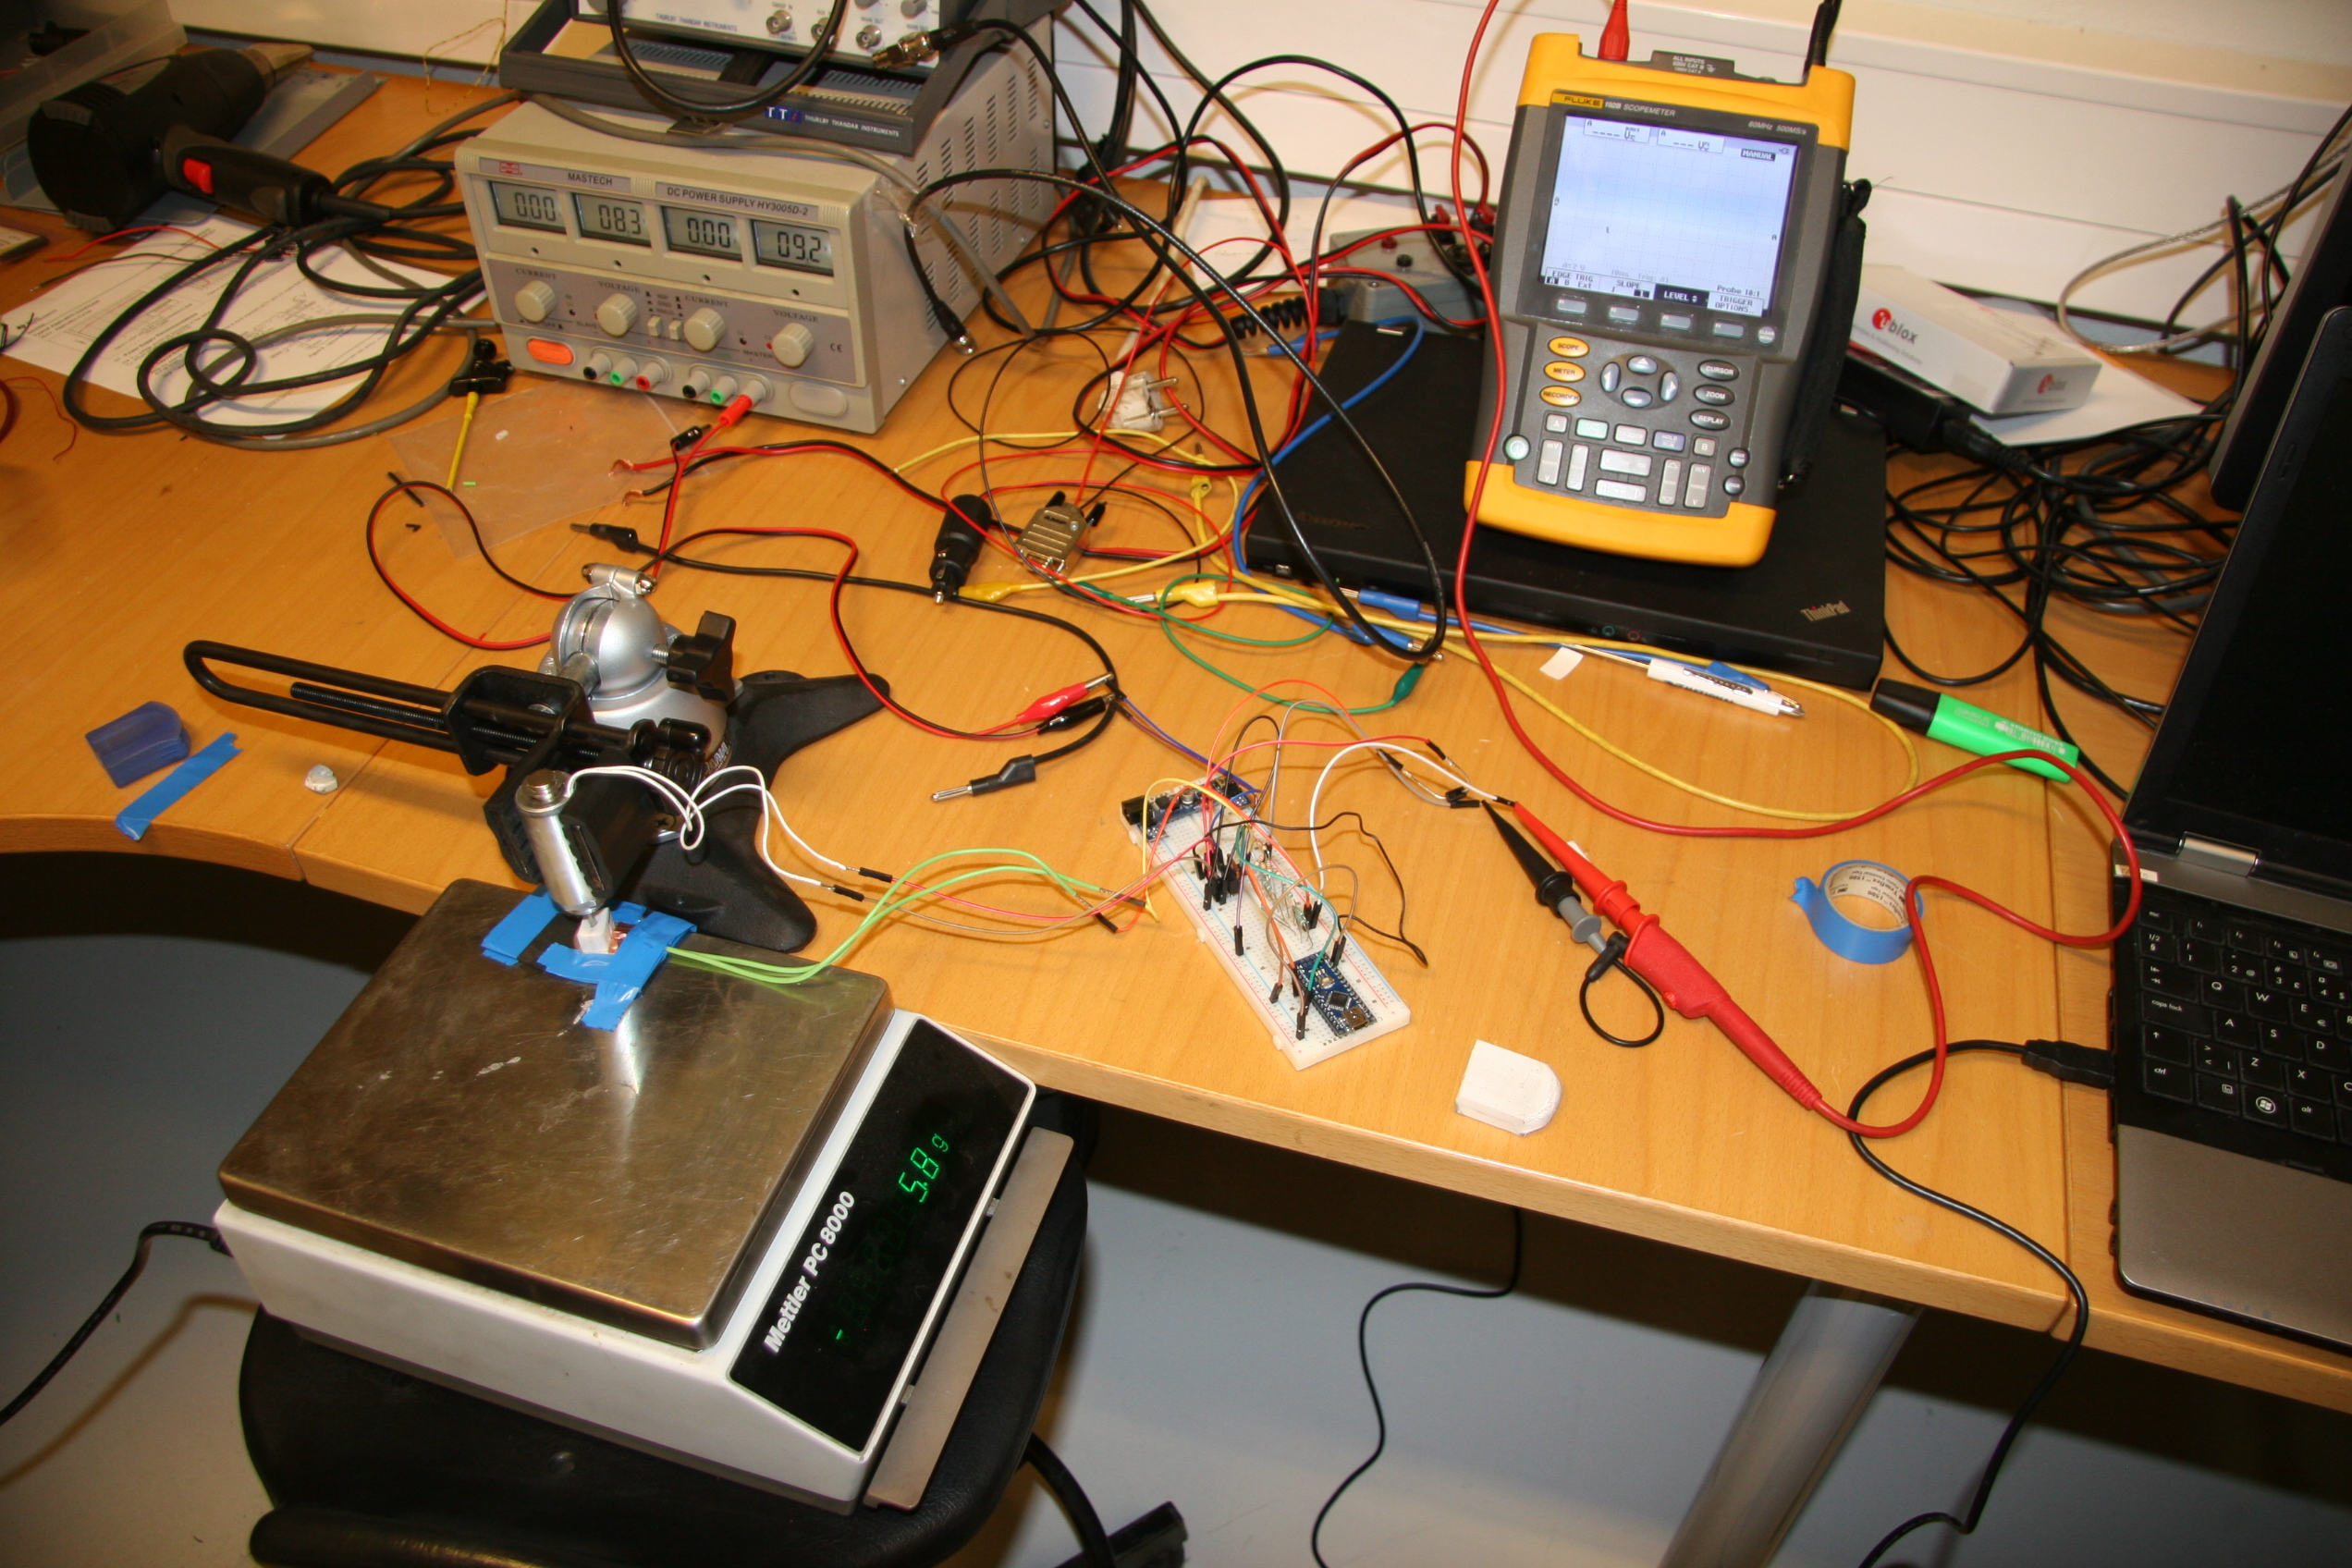
\includegraphics[height=4cm]{images/own_pic/piezo_test}
  \end{center}
  \caption{Test platform for piezo characteristics.}
  \label{fiq:piezo_impact}
\end{figure}

The measurement results are shown in figure \ref{fiq:piezo_measurement_chart}. Output voltage scales with square of impact force, which makes sense as work done can be expressed as $W = F * d$, where $W$ is work, $F$ is force and $d$ is distance force acts on object. As the displacement of piezo grows with the applied force, total work and therefore energy grows with both terms. 

\begin{figure}[htb]
  \begin{center}
  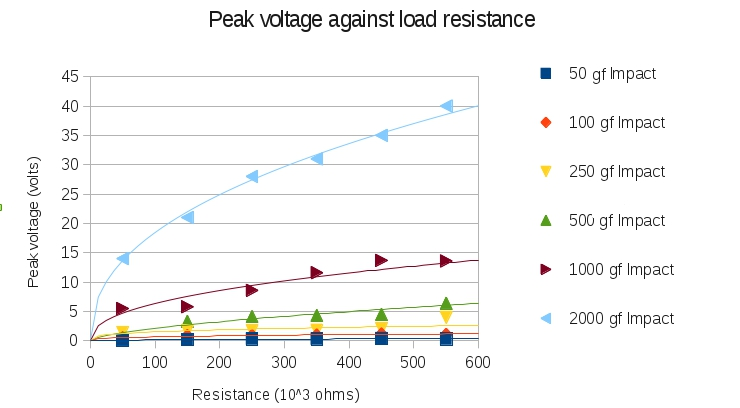
\includegraphics[height=4cm]{images/own_measurement/piezo_measurements}
  \end{center}
  \caption{Measured output voltage at different loads and impact forces.}
  \label{fiq:piezo_measurement_chart}
\end{figure}

Peak voltage grows with the load resistance. This makes sense in both voltage source and current source models, as the capacitor starts to discharge through load resistance instantly when voltage is applied over it. The relationship between voltage and load resistance seems to be logartithmic, which would be in good agreement with the logarithmic discharge curve of capacitor-resitor system. Peak voltages were read out from digital display and they can be considered reasonably accurate.

The time constants for voltage halving was graphically measured from oscilloscope waveforms, and this data was used to calculate the capacitance of TH-5C. These measurements are a lot less accurate, as readouts from oscilloscope screen have resolution of approximately half of line division, leaving accuracy of measurements at $\pm 2.5 ms$. These results are plotted in figure \ref{fig:piezo_time_capacitance}

\begin{figure}[htb]
  \begin{center}
  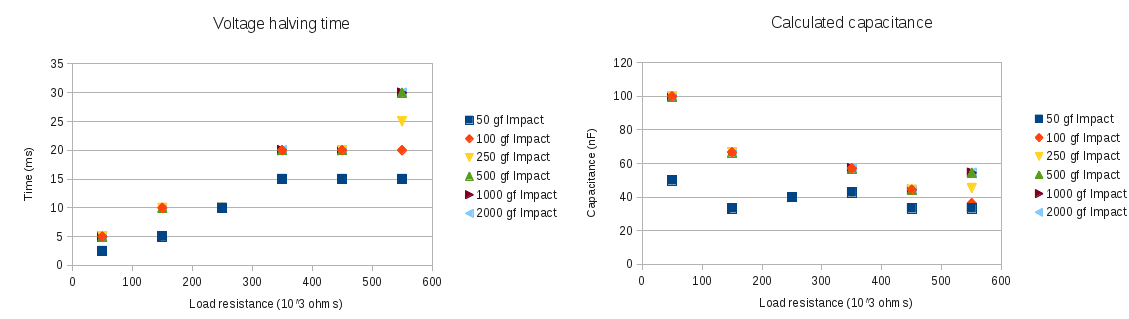
\includegraphics[height=4cm]{images/own_measurement/piezo_capacitance}
  \end{center}
  \caption{Measured half-time of system and calculated capacitance of piezo.}
  \label{fig:piezo_time_capacitance}
\end{figure}

The half-time data can be used to calculate capacitance of piezo using the RC-time constant of circuit:

\begin{equation}
  C=\frac{t}{-ln(\frac{1}{2})R} 
\end{equation}

 TH-5C provides value of 39nF as the capacitance, while these calculated values are notably higher and rise with the loading of piezo. Most likely explanation of this observation is the mechanical response time of system: solenoid plunger will take some milliseconds to reach new force equiliberium, and this effect becomes more pronounced at smaller time constants of RC-system. 
 
 {\color{red}TODO: Determine risetime from experimental data, compare to values given in solenoid datasheet}

 Using the known voltages, time constants and load resistances power and energy in impact can be determined:
 
 \begin{equation}
   TODO
\end{equation}
 
 The calculations are plotted in graph \ref{fig:piezo_power_energy}. As these calculations are based on inaccurately measured time, they should not be used as reference for any further calculations. However, trends can be seen in these values. 
 
 Interestingly the peak work done by piezo to resistor seems to be almost constant on all load levels. This is probably a consequence of logartithmic voltage-load relationship described above. There is a possibly significant result based on these findings: total energy obtainable from harvester grows with load resistance. However, this is applicable only for resistive load under impact-based energy generation.
 
 \begin{figure}[htb]
  \begin{center}
  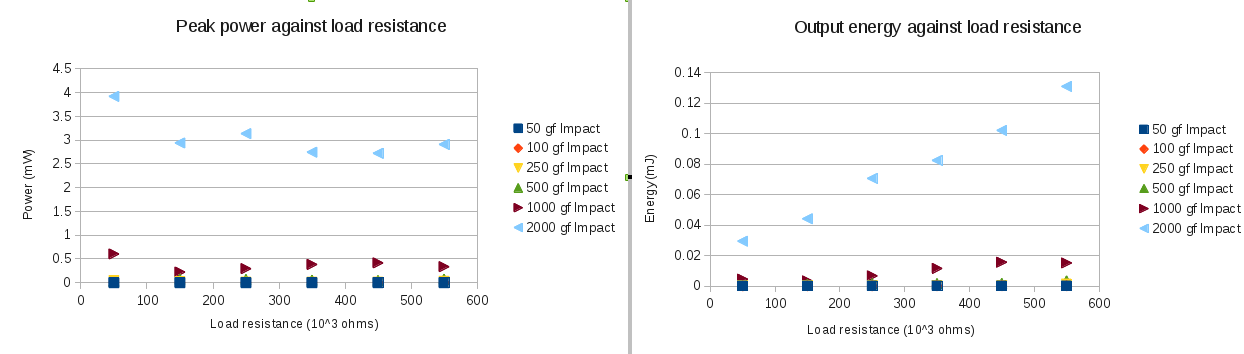
\includegraphics[height=4cm]{images/own_measurement/piezo_power}
  \end{center}
  \caption{Calculated piezo power and energy output}
  \label{fig:piezo_power_energy}
\end{figure}

Based on these results, an electrical equivalent model of circuit was designed. The model is shown in figure \ref{fig:piezo_ltspice_equivalent}. Model has two parallel current sources, one to simulate impact of on piezo and other to simulate release of the impact. Capacitance in parallel is set to 39 nF as given in datasheet, load resistance is parametrised to step through the experimental values. 

Model was tuned by first calculating the total current transfer to reach the open circuit voltage over capacitor. Then rise times of current sources were adjusted until simulated data matched experimental data.
The simulated data is plotted with experimental data in figure \ref{fiq:piezo_simulation_experimental}.

 \begin{figure}[htb]
  \begin{center}
  \includegraphics[height=4cm]{images/own_pic/piezo_equivalent_model}
  \end{center}
  \caption{Equivalent model of piezo}
  \label{fig:piezo_ltspice_equivalent}
\end{figure}

 \begin{figure}[htb]
  \begin{center}
  \includegraphics[height=4cm]{images/own_pic/piezo_sim_validation}
  \end{center}
  \caption{Simulated data compared to experimental results}
  \label{fiq:piezo_simulation_experimental}
\end{figure}

The experimental and simulated data are in good agreement. The simulation can be used as basis for modeling the behaviour of piezoelectronic element for the purposes of experimenting with maximum power point tracking algorithms as well as to estimate circuit efficiencies.

\subsubsection{Electromagnetical harvesting}
Electromagnetical harvesting is based on Faraday's law of induction: A loop of wire acquires electromotive force (EMF) in response to a changing magnetic field. More formally:

\begin{equation}
  \varepsilon = - \frac{d \Phi_ {B}}{d t} , 
\end{equation}

where $\varepsilon$ is the EMF, $\Phi_{B}$ is magnetic flux through loop area, and $t$ is time. Negative sign signifies that emf opposes the change of magnetic flux. For a tightly wound coil of wire, the equation can be stated as: 

\begin{equation} \label{eq:emf}
  \varepsilon = -N_{turns} \frac{d \Phi_{B}}{d t} , 
\end{equation}

where $N_{turns}$ is the number of turns in a coil. \cite[p.999]{universityphysics}

It's important to notice that magnetic flux through wire $ \Phi_{B} $ can change for a variety of reasons: the source of field can be in motion, strength of field can vary, the coil can be in motion, and the shape of coil can vary. In an energy harvesting application in an environment with vibrations motional energy is readily available, so we focus on energy harvesting methods which either move the source of magnetic field or the coil itself.

It can be determined from equation \eqref{eq:emf} that the energy available increases with the strength of magnetic source, number of turns in a coil and rate of change in the magnetic field. 

Magnetic source can be either a permanent magnet or an electrically induced source as in induction motors. Induction-based generators require reactive power to start up, which means that any harvester design incorporating an induction generator would need a secondary power source to start the inductive generator. Hence the focus of this thesis will be in permanent magnet designs.

In addition to voltage available from the generator, it's important to consider the source impedance. A very simple electrical equivalent model of the generator is presented in figure \ref{gen_simple}, where generator is presented as a voltage source in series with lumped inductor and resistor \cite{Jirutitijaroen2012}. 

\begin{figure}[htb]
\begin{center}
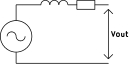
\includegraphics[height=2cm]{images/own_dwg/gen_simple}
\end{center}
\caption{A simple electromachanical generator equivalent circuit.}.
\label{gen_simple}
\end{figure}

This model is greatly simplified and it does not account for factors such as effect of electromagnetical force on mechanical structure of the generator. Even with these limitations, the model is still useful as it can be used to determine an optimal load for the generator. 

The power output can be written formally as:

\begin{equation} \label{eq:gen_simple_power}
  P_{generated}(s) = \varepsilon(s)*I_{generated}(s),
\end{equation}

where $P_{generated}(s), \varepsilon(s), I_{generated}(s)$ are complex frequency-domain power, voltage and current dependent. Voltage is determined by EMF as described above. Current can be written as: 

\begin{equation} \label{eq:gen_simple_current}
  I_{generated}(s) = \frac{\varepsilon(s)}{Z_{generator}(s)+Z_{load}(s)},
\end{equation}

where $Z_{generator}(s) $ and $ Z_{load}(s)$ are complex impedances of load and generator. This equation is valid only for linear systems, so for example rectifying and converting power with switch-mode power supply (SMPS) reduces accuracy of the equation. Substituting \eqref{eq:gen_simple_current} into \eqref{eq:gen_simple_power} we obtain:

\begin{equation}
  P_{generated}(s) = \varepsilon(s)*\frac{\varepsilon(s)}{Z_{generator}(s)+Z_{load}(s)}.
\end{equation}

Total power into load can be written as:

\begin{equation} \label{eq:generator_load_power}
  P_{load}(s) = \varepsilon(s)*\frac{Z_{load}(s)}{Z_{generator}(s)+Z_{load}(s)}*\frac{\varepsilon(s)}{Z_{generator}(s)+Z_{load}(s)}.
\end{equation}

It's easy to see from \eqref{eq:generator_load_power} that if the load impedance is infinite or zero, there is no power generated. It can be shown that maximum power is generated when load impedance is complex conjugate of generator impedance, $Z_{generator}(s) = {Z_{load}(s)}^*$. Another consideration is efficiency of the generator: the electrical efficiency is defined as ratio of power flowing into load and total power generated. Equation \eqref{eq:generator_load_power} can be used to show that when load impedance is equal to generator impedance, efficiency is $ 50 \%$. Efficiency rises with the load impedance, which is why generators are rarely run at their maximum power. In our application the harvested power is minuscule compared to power available in tyre, so it makes sense to try to match the load impedance for maximum power.

In an energy harvesting application it is important to consider the validity of established theory when generator is scaled to centimetres or even smaller dimensions. Many assumptions, such as coil being tightly wound and made of thin wire might become invalid at microscale. O'Donnel et al. \cite{ODonnell2007} have done a study on the effects of scaling dimensions downwards down to millimetre range, and they concluded that power available from generator is proportional to fourth power of generator dimension for cubical generators. Another of their primary findings was that a microfabricated generator becomes more effective than a traditional wire-wound generator when design is scaled below $2 mm$ length or in $8 mm^3$ volume. It can be concluded that in this application it is reasonable to use a wire-wound generator over microfabricated one, as the generator dimensions can be an order of magnitude larger than this crossover point. 

\begin{comment}

\subsubsection{Magnetostrictive harvesting}
TODO: Magnetostrictive harvesting resembles piezoelectric harvesting. Figure \ref{magneto} shows proposed system, where magnetostrictive cantilever is sandwiched between biasing magnets and a pickup coil.  

\begin{figure}[htb]
\begin{center}
\includegraphics[height=4cm]{images/cited/magneto}
\end{center}
\caption{A magnetostrictive energy harvester by Wang et al. \cite{Wang2006}}.
\label{magneto}
\end{figure}



\subsection{Powering the sensor}
Traditionally wireless sensors have been powered with either primary or rechargeable batteries. These systems need service at regular intervals to change or recharge the batteries. In applications where battery cannot be accessed, battery lifetime often limits the lifetime of whole system. Alternative approach has been to use generators, such as fuel cells or even radioactive power sources. These systems often have a poor power density and decreasing efficiency when scaled down to small size \cite{Knight2008}. 

This work explores ways to utilise energy present in tyre to power the sensor itself. A single tyre can waste as much as 500 W of power at high speeds {\color{red} source}, so harvesting even 1/100 000ths of wasted power would be enough for a well designed low-power sensor and transmitter.

There are many different energy harvesting solutions which use fundamentally different physical principles and energy sources, such as thermal, solar, radio waves and mechanical. {\color{red} source}. As the energy harvester is inside tyre, solar harvesting is unfeasible. Radio wave harvesting methods rely on external radio transmissions for gathering power. As the device should work regardless of external environment, these methods are not suited for application. Thermal methods require significant temperature gradients {\color{red} source}, but previous work shows that car tyre can reach only ambient plus few tens of \degree C {\color{red} source}. Therefore thermal methods would be ineffective. 

Mechanical energy harvesting is a natural choice, as there is abundant amount of mechanical energy available as accelerations, vibrations and centripetal force available inside the tyre. There are various different approaches for harvesting mechanical energy, including piezoelectronic, electrostatic, electromagnetic and microelectromechanical systems (MEMS) {\color{red} source}. To select optimal method for energy harvesting, more information about the characteristics of mechanical energy is required.

{\color{yellow} refer to \cite[p.10]{Kubba2014}}

The power requirements of system create additional constraints on energy harvesting method, as the energy harvester must be able to supply enough energy and power to system. In a real-world application the power management system must be able to store energy for some period of time so sensor can operate continuosly. 




As the electromagnetical harvester does not bend in any direction, it's better suited to be built straight up along Z-axis. The structure can be made strong enough to survive the shocks present without compromising on the harvester operation. A magnet can be suspended with a spring inside a coil, or by using another magnet in a repulsing configuration as presented by Torincasa et al. \cite{Tornincasa2012}. When there is vibration in addition to relatively constant centripetal force, the magnet will move along the shaft of the coil and generate electricity. Figure \ref{lgm} shows the structure of built generator. 

A non-linear spring can be utilised to keep the magnet as well centered as possible over a wide range of tyre speeds. Theoretically this non-linearity could also be used to shift the resonant frequency of generator to track the frequency of vibration inside the tyre. In practise the movement of magnet would drive the spring outside of the resonant area. 
\end{comment}
